\documentclass[11pt,a4paper,oneside]{article}
\usepackage[margin=26mm,headheight=15pt,footskip=12mm]{geometry}
\usepackage{fontspec}\setmainfont{Latin Modern Roman}
\usepackage[danish]{babel}\usepackage{amsmath,amssymb,mathtools,booktabs,array,microtype,xcolor,tikz,pgfplots,fancyhdr,hyperref,titlesec,enumitem,longtable}
\pgfplotsset{compat=1.18}
\definecolor{accent}{HTML}{315D77}\definecolor{rulegray}{HTML}{CFD8DD}
\hypersetup{colorlinks=true,linkcolor=accent,bookmarksnumbered=true,pdfauthor={Fysik-studiearkiv},pdftitle={Analytisk Mekanik – Formelsamling}}
\setlength{\parindent}{0pt}\setlength{\parskip}{7pt}\setlength{\emergencystretch}{3em}
\pagestyle{fancy}\fancyhf{}\fancyhead[L]{\small\sffamily\bfseries Analytisk mekanik}\fancyhead[R]{\small\color{accent} Formelsamling}\fancyfoot[L]{\footnotesize Definitioner \textperiodcentered\ metode \textperiodcentered\ kontrol}\fancyfoot[R]{\footnotesize\thepage}\renewcommand{\headrulewidth}{0.35pt}
\titleformat{\section}{\Large\bfseries\color{accent}}{\thesection}{0.9em}{}[\vspace{-3pt}\color{rulegray}\titlerule]
\titleformat{\subsection}{\large\bfseries}{\thesubsection}{0.65em}{}
\titlespacing*{\section}{0pt}{17pt}{10pt}\titlespacing*{\subsection}{0pt}{15pt}{6pt}
\newcommand{\dd}{\mathrm d}\newcommand{\pd}[2]{\frac{\partial #1}{\partial #2}}\newcommand{\od}[2]{\frac{\dd #1}{\dd #2}}\newcommand{\vv}[1]{\boldsymbol{#1}}\newcommand{\PB}[2]{\left\{#1,#2\right\}}
\newcommand{\key}[1]{\par\medskip\begingroup\color{accent}\rule{\linewidth}{0.4pt}\par\vspace{3pt}\color{black}\ensuremath{\displaystyle #1}\par\vspace{3pt}\color{accent}\rule{\linewidth}{0.4pt}\endgroup\medskip}
\newenvironment{method}{\par\smallskip\noindent\textbf{Fremgangsmåde.}\ }{\par\smallskip}
\newenvironment{note}{\par\smallskip\noindent\textcolor{accent}{\textbf{Bemærk.}}\ }{\par\smallskip}
\begin{document}

{\huge\bfseries Analytisk Mekanik}\par\vspace{5pt}
{\Large\color{accent}Formelsamling og opgavemetoder}\par\medskip
\textit{Definitioner, anvendelige komponentformler og sammenhængende metoder.}
\vspace{5pt}\tableofcontents\clearpage
\clearpage\section{Generaliserede koordinater og mekaniske størrelser}\label{sec:gen-coordinates}
\textbf{Fysisk problem.} Før vi kan udlede en bevægelsesligning, må vi beskrive systemets mulige positioner, bevægelser og kræfter korrekt. Vi går fra bindinger og koordinatvalg til hastigheder, energi og impulser og slutter med en Lagrangefunktion $\mathcal L(q,\dot q,t)$, som anvendes i kapitel~2.

\subsection{Frihedsgrader, bindinger og koordinatvalg}
Et system af $N$ punktpartikler i tre dimensioner har oprindeligt $3N$ kartesiske koordinater. Har det $k$ \emph{uafhængige, regulære holonome} bindinger $f_\alpha(\vv r_1,\dots,\vv r_N,t)=0$, er antallet af lokale frihedsgrader
\key{n=3N-k.}
Formlen gælder ikke uden videre for vilkårlige hastighedsbindinger eller afhængige bindinger. \emph{Holonome} bindinger kan udtrykkes som ligninger mellem positioner og eventuelt tid; ikke-holonome bindinger kan generelt ikke integreres til sådanne ligninger. \emph{Skleronom} betyder uden eksplicit tid; \emph{reonom} betyder eksplicit tidsafhængig.
\begin{center}\small
\begin{tabular}{p{36mm}p{54mm}p{48mm}}\toprule
System & Binding & Mulige frie koordinater\\\midrule
Partikel på cirkel & $x^2+y^2=R^2$ & $\phi$\\
Partikel på kugle & $x^2+y^2+z^2=R^2$ & $(\theta,\phi)$\\
Simpelt pendul i plan & $x^2+y^2=l^2$ & $\theta$\\\bottomrule
\end{tabular}\end{center}
\textbf{Pendul som gennemgående eksempel.} Lad ophængspunktet være origo, $y$ pege opad, og længden være $l>0$. Vælg
\[
x=l\sin\theta,\qquad y=-l\cos\theta.
\]
Bindingen $x^2+y^2=l^2$ er dermed opfyldt identisk. I stedet for at løse for to afhængige variable $(x,y)$ kan vi arbejde med én uafhængig vinkel $\theta$. En generaliseret koordinat er altså \emph{enhver} egnet parameter for konfigurationsrummet, ikke nødvendigvis en længde.

Et koordinatkort skal være lokalt uafhængigt og regulært. For et kvadratisk skift $Q_i=Q_i(q,t)$ med samme dimension er den lokale invertibilitet sikret af
\[
\boxed{\det\left(\frac{\partial Q_i}{\partial q_j}\right)\ne0.}
\]
Mere generelt kræves, at koordinatparametriseringen har fuld rang. Et polært kort bliver eksempelvis singulært i $r=0$. Dette er en \emph{koordinatbetingelse}, ikke kanonicitetstesten for en transformation i faserummet (se afsnit~\ref{sec:canon}).
\begin{method}Optæl uafhængige bindinger; vælg $n$ uafhængige $q_i$; skriv hver partikelposition $\vv r_a(q,t)$; kontrollér bindinger og eventuelle koordinatsingulariteter, før hastigheder og energi beregnes.\end{method}

\subsection{Koordinattransformationer, hastigheder og accelerationer}
Lad $\vv r_a=\vv r_a(q_1,\ldots,q_n,t)$ være positionen af partikel $a$. Langs den faktiske bane bliver $\vv r_a$ tidsafhængig både gennem $q_i(t)$ og gennem en mulig eksplicit tidsafhængighed. Kædereglen giver
\key{\dot{\vv r}_a=\sum_{i=1}^n
\frac{\partial\vv r_a}{\partial q_i}\dot q_i+
\left.\frac{\partial\vv r_a}{\partial t}\right|_q.}
I $\partial\vv r_a/\partial q_j$ holdes de andre koordinater og tiden faste; i $\partial\vv r_a/\partial t|_q$ holdes alle $q_i$ faste. Punktet angiver derimod den \emph{totale} tidsafledte langs $q_i(t)$.
Fordi $\dot q_i$ betragtes som uafhængige argumenter i tangentbundtet, følger direkte
\key{\frac{\partial\dot{\vv r}_a}{\partial\dot q_j}
=\frac{\partial\vv r_a}{\partial q_j}.}
Differentieres hastigheden endnu en gang, fås
\[
\ddot{\vv r}_a=
\sum_i\frac{\partial\vv r_a}{\partial q_i}\ddot q_i+
\sum_{i,j}\frac{\partial^2\vv r_a}{\partial q_i\partial q_j}\dot q_i\dot q_j+
2\sum_i\frac{\partial^2\vv r_a}{\partial t\partial q_i}\dot q_i+
\left.\frac{\partial^2\vv r_a}{\partial t^2}\right|_q.
\]
Denne form forudsætter tilstrækkeligt glatte transformationer; ved tidsafhængige og roterende referencebaser er det særligt vigtigt at differentiere basisvektorerne (kapitel~4).

\textbf{Eksamen 2023, opgave 4a:} Betragt den lokale punkttransformation
\[
x=\tfrac12(u^2-v^2),\qquad y=uv.
\]
Da koordinatskiftet ikke afhænger eksplicit af tiden, giver kædereglen
\[
\dot x=u\dot u-v\dot v,\qquad
\dot y=v\dot u+u\dot v.
\]
Og dermed
\[
\frac{\partial\dot x}{\partial\dot u}=u,\quad
\frac{\partial\dot x}{\partial\dot v}=-v,\quad
\frac{\partial\dot y}{\partial\dot u}=v,\quad
\frac{\partial\dot y}{\partial\dot v}=u.
\]
Jacobideterminanten er $u^2+v^2$; den er positiv bortset fra $(u,v)=(0,0)$. Skiftet er derfor lokalt invertibelt væk fra origo, men globalt er $(u,v)$ og $(-u,-v)$ samme punkt i $(x,y)$.
\begin{method}Skriv først de gamle koordinater som funktioner af de nye og tiden; anvend kædereglen på hver koordinat; differentier med hensyn til én $\dot q_j$ ad gangen, mens alle øvrige $q,\dot q,t$ fastholdes. Kontrollér eventuelt Jacobien.\end{method}

\subsection{Kinetisk energi, potentiale og Lagrangefunktionen}
For punktmasser i et inertielt kartesisk system er
\[
T=\frac12\sum_a m_a\dot{\vv r}_a\cdot\dot{\vv r}_a.
\]
Indsæt de transformerede hastigheder for at få $T(q,\dot q,t)$. Den generaliserede kinetiske energi behøver ikke være summen af udtryk $\frac12m\dot q_i^2$; der kan være metrikkens faktorer, krydsled og ved reonome koordinater også hastighedslineære led.

I plan polære koordinater er $\vv r=r(\cos\phi,\sin\phi)$ og
\[
\dot x=\dot r\cos\phi-r\dot\phi\sin\phi,\qquad
\dot y=\dot r\sin\phi+r\dot\phi\cos\phi.
\]
Krydsleddene ophæves i $\dot x^2+\dot y^2$, så
\key{T=\frac12m(\dot r^2+r^2\dot\phi^2).}
For pendulet indsættes $x=l\sin\theta$, $y=-l\cos\theta$:
\[
\dot x=l\cos\theta\,\dot\theta,\quad
\dot y=l\sin\theta\,\dot\theta,\quad
T=\frac12ml^2\dot\theta^2.
\]
En \emph{konservativ} kraft kan lokalt skrives $\vv F=-\nabla V$. I én dimension er $F_x=-\mathrm dV/\mathrm dx$, altså $V(x)=-\int F_x(x)\,\dd x+C$. I flere dimensioner kræver et potentiale passende integrabilitetsbetingelser og domæneforhold; en hastighedsafhængig friktionskraft er ikke en almindelig konservativ potentialkraft. For pendulet er $V=mgy=-mgl\cos\theta$ (additive konstanter kan udelades). Derfor
\[
\boxed{\mathcal L=T-V=\frac12ml^2\dot\theta^2+mgl\cos\theta.}
\]
Her stopper vi ved \emph{opstillingen} af systemet; Euler--Lagrange giver bevægelsesligningen i næste kapitel.

\subsection{Generaliseret impuls og impulsens transformation}
Den impuls, som er konjugeret til $q_i$, defineres ved
\key{p_i=\frac{\partial\mathcal L}{\partial\dot q_i}.}
Den er ikke nødvendigvis en komponent af kartesisk lineær impuls. For $T=\frac12m(\dot r^2+r^2\dot\phi^2)$ og hastighedsuafhængigt potentiale fås
\[
p_r=m\dot r,\qquad p_\phi=mr^2\dot\phi.
\]
$p_\phi$ er et impulsmoment, mens $p_r$ er radial impuls; begge har de enheder, som følger af deres tilhørende koordinater. For eksempel er pendulets $p_\theta=ml^2\dot\theta$.

\textbf{Punkttransformation:} Lad de gamle koordinater $x_i$ være givet ved $x_i=x_i(Q,t)$, og antag en regulær transformation samt en Lagrangefunktion, der blot omskrives ved substitution, $\mathcal L'(Q,\dot Q,t)=\mathcal L(x(Q,t),\dot x(Q,\dot Q,t),t)$. Kædereglen og hastighedsidentiteten giver
\[
P_j=\frac{\partial\mathcal L'}{\partial\dot Q_j}
=\sum_i\frac{\partial\mathcal L}{\partial\dot x_i}
\frac{\partial\dot x_i}{\partial\dot Q_j}
=\boxed{\sum_i p_i\frac{\partial x_i}{\partial Q_j}}.
\]
Dette er transformationen af \emph{kanoniske} impulskomponenter for punkttransformationer; hastighedsafhængige potentialer ændrer definitionen af $p_i$, og en ekstra total tidsafledt i Lagrangefunktionen kan forskyde impulserne.

For koordinatskiftet fra 2023.4a bliver
\[
\boxed{p_u=up_x+vp_y,\qquad p_v=-vp_x+up_y.}
\]
\begin{method}Skriv gamle koordinater som funktion af nye; beregn Jacobimatricen $\partial x_i/\partial Q_j$; transformér impulserne med dens transponerede matrix. Kontrollér, at alle termer og enheder passer, samt hvor Jacobien er invertibel.\end{method}

\subsection{Generaliserede kræfter og virtuelt arbejde}
En \emph{virtuel forskydning} $\delta\vv r_a$ er en infinitesimal ændring i konfigurationen ved fast tid, der respekterer de valgte holonome bindinger:
\[
\delta\vv r_a=\sum_i\frac{\partial\vv r_a}{\partial q_i}\delta q_i.
\]
For påførte fysiske kræfter fås virtuelt arbejde
\[
\delta W=\sum_a\vv F_a\cdot\delta\vv r_a
=\sum_i\underbrace{\left(\sum_a\vv F_a\cdot
\frac{\partial\vv r_a}{\partial q_i}\right)}_{\mathcal Q_i}\delta q_i.
\]
Derfor er
\key{\mathcal Q_i=\sum_a\vv F_a\cdot
\frac{\partial\vv r_a}{\partial q_i},\qquad
\mathcal Q_i^{\rm kons}=-\frac{\partial V}{\partial q_i}.}
Dette er \emph{generaliseret kraft}, ikke en ny koordinat $Q_i$; store $Q_i$ bruges senere om nye kanoniske koordinater. Enheden bestemmes af $\delta W=\mathcal Q_i\delta q_i$: for en længde er den newton, for en dimensionsløs vinkel er den newtonmeter.

Ved ideelle bindinger gør bindingskræfterne intet virtuelt arbejde. D'Alemberts princip udtrykker da
$\sum_a(\vv F_a-m_a\ddot{\vv r}_a)\cdot\delta\vv r_a=0$,
hvilket er et andet udgangspunkt for Lagrangeformalismen; den fulde udledning via stationær virkning følger i kapitel~2. For ikke-ideelle bindinger skal de ikke-nul virtuelle bindingsarbejder medtages særskilt.

\subsection{Samlet opstilling: det simple pendul}
Et punktlegeme med masse $m$ hænger i en masseløs, ustrækkelig snor af længde $l$ i et homogent tyngdefelt. Den regulære binding begrænser bevægelsen til én vinkel $\theta$:
\[
(x,y)=(l\sin\theta,-l\cos\theta)
\ \Rightarrow\
(\dot x,\dot y)=(l\cos\theta\,\dot\theta,l\sin\theta\,\dot\theta).
\]
Dermed
\[
T=\frac12ml^2\dot\theta^2,\quad V=-mgl\cos\theta,\quad
\boxed{\mathcal L=\frac12ml^2\dot\theta^2+mgl\cos\theta},\quad
p_\theta=ml^2\dot\theta.
\]
Bemærk, at $p_\theta$ ikke er en kartesisk impuls; og at bindingen allerede er elimineret med koordinatvalget. Bevægelsesligningen udledes først i afsnit~2.2.
\begin{method}\textbf{Fra opgavetekst til $\mathcal L$:} (1) find system og bindinger, (2) vælg uafhængige $q_i$, (3) skriv $\vv r_a(q,t)$ og $\dot{\vv r}_a$, (4) beregn $T$ og $V$, (5) opstil $\mathcal L=T-V$, (6) find eventuelt $p_i=\partial\mathcal L/\partial\dot q_i$. Kontrollér enheder, koordinatdomæne og alle bindingsrelationer.\end{method}

\clearpage\section{Lagrangeformalismen og bevarelseslove}\label{sec:lagrange}
\textbf{Fra opstilling til bevægelse.} I kapitel~1 valgte vi uafhængige koordinater, beregnede $T,V$ og opstillede $\mathcal L(q,\dot q,t)$. Hvordan bestemmes nu $q_i(t)$? Vi begynder med Hamiltons princip, udleder Euler--Lagrange og bruger derefter symmetrier, energi og bindinger til at reducere arbejdet.

\subsection{Virkningen og Hamiltons princip}
Til en mulig bane $q_i(t)$ mellem to faste tidspunkter $t_1,t_2$ knyttes virkningen
\[
S[q]=\int_{t_1}^{t_2}\mathcal L(q,\dot q,t)\,\dd t.
\]
Hamiltons princip siger, at den fysiske bane gør virkningen \emph{stationær}: $\delta S=0$ for alle tilstrækkeligt små variationer med faste endepunkter,
$\delta q_i(t_1)=\delta q_i(t_2)=0$. Stationær betyder ikke nødvendigvis et minimum.

Skriv $q_i(t,\varepsilon)=q_i(t)+\varepsilon\eta_i(t)$, hvor $\eta_i(t_1)=\eta_i(t_2)=0$. Den første variation er
\[
\delta S=\int_{t_1}^{t_2}\sum_i\left(
\frac{\partial\mathcal L}{\partial q_i}\delta q_i+
\frac{\partial\mathcal L}{\partial\dot q_i}\delta\dot q_i
\right)\dd t.
\]
Da $\delta\dot q_i=\dd(\delta q_i)/\dd t$, kan det andet led integreres ved dele:
\begin{align*}
\int_{t_1}^{t_2}\frac{\partial\mathcal L}{\partial\dot q_i}
\frac{\dd(\delta q_i)}{\dd t}\,\dd t
&=\left[\frac{\partial\mathcal L}{\partial\dot q_i}\delta q_i\right]_{t_1}^{t_2}
-\int_{t_1}^{t_2}\frac{\dd}{\dd t}
\left(\frac{\partial\mathcal L}{\partial\dot q_i}\right)\delta q_i\,\dd t\\
&=-\int_{t_1}^{t_2}\frac{\dd}{\dd t}
\left(\frac{\partial\mathcal L}{\partial\dot q_i}\right)\delta q_i\,\dd t,
\end{align*}
fordi randleddet er nul. Dermed
\[
\delta S=\int_{t_1}^{t_2}\sum_i\left[
\frac{\partial\mathcal L}{\partial q_i}-
\frac{\dd}{\dd t}\left(\frac{\partial\mathcal L}{\partial\dot q_i}\right)
\right]\delta q_i\,\dd t.
\]
Variationerne er vilkårlige indvendigt i tidsintervallet, så hver koefficient må forsvinde. Vi har således udledt Euler--Lagrange-ligningerne:
\key{\frac{\dd}{\dd t}\left(\frac{\partial\mathcal L}{\partial\dot q_i}\right)
-\frac{\partial\mathcal L}{\partial q_i}=0.}
Udledningen forudsætter tilstrækkeligt glat $\mathcal L$ og uafhængige variationer af de valgte generaliserede koordinater. En alternativ håndtering af bindinger er multiplikatormetoden i afsnit~\ref{sec:lambda}.

\subsection{Euler--Lagrange som fremgangsmåde}
Definér den generaliserede impuls $p_i=\partial\mathcal L/\partial\dot q_i$. Den lokale ligning er
$\dd p_i/\dd t=\partial\mathcal L/\partial q_i$; dette er ikke en påstand om, at $p_i$ generelt er bevaret.
For pendulet fra kapitel~1 har vi
\[
\mathcal L=\frac12ml^2\dot\theta^2+mgl\cos\theta,\quad
\frac{\partial\mathcal L}{\partial\dot\theta}=ml^2\dot\theta,\quad
\frac{\partial\mathcal L}{\partial\theta}=-mgl\sin\theta.
\]
Derfor
\[
ml^2\ddot\theta+mgl\sin\theta=0
\quad\Longrightarrow\quad
\boxed{\ddot\theta+\frac gl\sin\theta=0.}
\]
Dette er en \emph{differentialligning} for $\theta(t)$, ikke selve tidsløsningen. Hvis en ikke-konservativ generaliseret kraft $\mathcal Q_i^{\mathrm{(nk)}}$ ikke allerede er beskrevet i $\mathcal L$, gælder i stedet
\[
\boxed{\frac{\dd}{\dd t}\frac{\partial\mathcal L}{\partial\dot q_i}
-\frac{\partial\mathcal L}{\partial q_i}=\mathcal Q_i^{\mathrm{(nk)}}.}
\]
Eksempelvis giver lineær dæmpning $\mathcal Q^{\mathrm{(nk)}}=-b\dot q$ med $b>0$ et ekstra led i ligningen; man må ikke behandle almindelig friktion som et konservativt $V(q)$.
\begin{method}Vælg $q_i$ og $\mathcal L$, udregn først $\partial\mathcal L/\partial\dot q_i$, differentier derefter \emph{totalt} efter tiden, og træk $\partial\mathcal L/\partial q_i$ fra. Indsæt eventuelle ikke-konservative generaliserede kræfter, kontroller dimensioner/fortegn, og anvend initialdata til løsningen.\end{method}

\subsection{Den harmoniske oscillator i én og to dimensioner}
For et kvadratisk potentiale i én dimension,
\[
\mathcal L=\frac12m\dot q^2-\frac12kq^2,\qquad m,k>0,
\]
giver Euler--Lagrange $m\ddot q+kq=0$. Sæt $\omega=\sqrt{k/m}$; ligningen har løsningen
\key{q(t)=A\cos(\omega t)+B\sin(\omega t).}
Givet $q(0)=q_0$ og $\dot q(0)=v_0$ bliver $A=q_0$ og $B=v_0/\omega$. En generel begyndelsestid $t_0$ håndteres tilsvarende ved at skrive løsningen med $(t-t_0)$.

For en isotrop oscillator i et plan er
\[
\mathcal L=\frac12m(\dot x^2+\dot y^2)-\frac12m\omega^2(x^2+y^2),
\quad \ddot x+\omega^2x=0,\ \ddot y+\omega^2y=0.
\]
Begge komponenter har samme frekvens:
\[
x=A\cos\omega t+B\sin\omega t,\qquad
y=C\cos\omega t+D\sin\omega t.
\]
Som vektorligning er $\vv r(t)=\vv a\cos\omega t+\vv b\sin\omega t$. Derfor er banen billedet af en enhedscirkel under den lineære afbildning med kolonnerne $\vv a$ og $\vv b$: i almindelighed en ellipse med centrum i origo. Er $\vv a$ og $\vv b$ lineært afhængige, degenererer ellipsen til et linjestykke; er de ortogonale med samme længde, bliver banen en cirkel.
\begin{center}
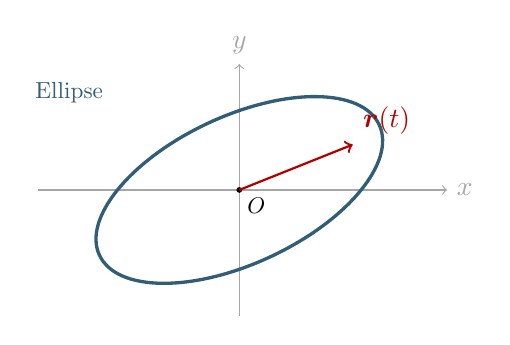
\begin{tikzpicture}[scale=.80]
\draw[->,gray!70](-3.2,0)--(3.3,0)node[right]{$x$};
\draw[->,gray!70](0,-2.0)--(0,2.0)node[above]{$y$};
\draw[accent,very thick,rotate=25] (0,0) ellipse (2.45 and 1.17);
\fill (0,0) circle (1.3pt) node[below right,scale=.82]{$O$};
\draw[->,thick,red!70!black] (0,0)--(1.8,.72) node[above right]{$\vv r(t)$};
\node[accent,scale=.84] at (-2.7,1.55){Ellipse};
\end{tikzpicture}
\end{center}
\textbf{Fortolkning.} Det er parameteren $t$, der gennemløber ellipsen; den særlige oscillator--Kepler-forbindelse senere i pensum anvender generelt \emph{ikke} den samme tidsparameter. Banens form alene afgør derfor ikke tidsudviklingen.
\begin{method}Genkend et kvadratisk potentiale, aflæs frekvensen, løs for hver uafhængig koordinat og fastlæg alle konstanter fra startposition og starthastighed. Ved koblede oscillatorer kan normalmodemetoder være nødvendige.\end{method}

\subsection{Symmetrier, cykliske koordinater og impulsmoment}\label{sec:angular}
\textbf{Kan vi finde bevarede størrelser uden at løse ligningerne?} Hvis $\mathcal L$ er uafhængig af en generaliseret koordinat $q_i$, siger Euler--Lagrange direkte
\[
\frac{\partial\mathcal L}{\partial q_i}=0
\quad\Longrightarrow\quad
\frac{\dd}{\dd t}\frac{\partial\mathcal L}{\partial\dot q_i}=0
\quad\Longrightarrow\quad \boxed{p_i=\mathrm{konstant}}.
\]
En sådan $q_i$ kaldes \emph{cyklisk}. Sammenhængen mellem symmetri og bevarelse er bredere: et kontinuerligt transformationsinvariant virkningsprincip giver Noether-bevarelseslove også i koordinater, hvor symmetrien ikke fremstår som en enkelt cyklisk variabel.
\begin{center}\small\renewcommand{\arraystretch}{1.17}
\begin{tabular}{p{40mm}p{49mm}p{51mm}}\toprule
Symmetri & Simpel lokal test & Bevaret størrelse\\\midrule
Translation i $x$ & $\partial\mathcal L/\partial x=0$ & $p_x=\partial\mathcal L/\partial\dot x$\\
Rotation om $z$ & $\partial\mathcal L/\partial\phi=0$ & $p_\phi=\partial\mathcal L/\partial\dot\phi$\\
Tidsforskydning & $\partial\mathcal L/\partial t=0$ & $h=\sum_i\dot q_i p_i-\mathcal L$\\\bottomrule
\end{tabular}\end{center}
I kartesiske inertielle koordinater med mekanisk impuls $\vv p=m\dot{\vv r}$ er impulsmomentet omkring origo
\key{\vv L=\vv r\times\vv p,\qquad
L_x=yp_z-zp_y,\quad L_y=zp_x-xp_z,\quad L_z=xp_y-yp_x.}
\begin{center}
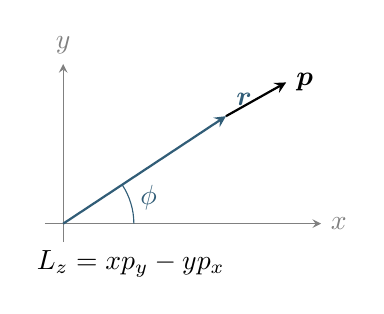
\begin{tikzpicture}[scale=.78,>=stealth]
\draw[->,gray](-.3,0)--(4.2,0)node[right]{$x$};
\draw[->,gray](0,-.3)--(0,2.6)node[above]{$y$};
\draw[->,thick,accent](0,0)--(2.65,1.75)node[above right]{$\vv r$};
\draw[->,thick](2.65,1.75)--(3.63,2.3)node[right]{$\vv p$};
\draw[accent](1.15,0) arc (0:33.4:1.15);
\node[accent] at (1.39,.42){$\phi$};
\node at (1.1,-.65){$L_z=xp_y-yp_x$};
\end{tikzpicture}
\end{center}
Ved en central kraft er drejningsmomentet $\vv\tau=\vv r\times\vv F=0$, så $\dd\vv L/\dd t=0$. I polære koordinater og uden ekstra hastighedsafhængige led er $L_z=p_\phi=mr^2\dot\phi$ for én partikel; for tolegemer bruges den reducerede masse i kapitel~\ref{sec:central}. Skeln mellem kanonisk og mekanisk impuls, hvor de ikke er ens.
\begin{method}Find koordinater, som ikke forekommer eksplicit i $\mathcal L$; differentier efter deres hastigheder for at få $p_i$. Ved rotationssymmetri: fastlæg akse, kontroller drejningsmoment eller cyklisk vinkel, og angiv den bevarede komponent af $\vv L$. Test symmetrien frem for automatisk at antage alle tre komponenter bevaret.\end{method}

\subsection{Energifunktionen og tidsinvarians}
Definér
\[
h(q,\dot q,t)=\sum_i\dot q_i\frac{\partial\mathcal L}{\partial\dot q_i}-\mathcal L.
\]
Differentier totalt:
\begin{align*}
\frac{\dd h}{\dd t}
&=\sum_i\left(\ddot q_i\frac{\partial\mathcal L}{\partial\dot q_i}
+\dot q_i\frac{\dd}{\dd t}\frac{\partial\mathcal L}{\partial\dot q_i}\right)
-\sum_i\left(\frac{\partial\mathcal L}{\partial q_i}\dot q_i
+\frac{\partial\mathcal L}{\partial\dot q_i}\ddot q_i\right)
-\frac{\partial\mathcal L}{\partial t}\\
&=\sum_i\dot q_i\left(\frac{\dd}{\dd t}
\frac{\partial\mathcal L}{\partial\dot q_i}
-\frac{\partial\mathcal L}{\partial q_i}\right)
-\frac{\partial\mathcal L}{\partial t}.
\end{align*}
På løsninger af Euler--Lagrange med ingen ikke-konservative ydre generaliserede kræfter forsvinder parenteserne, og derfor
\key{\frac{\dd h}{\dd t}=-\frac{\partial\mathcal L}{\partial t}.}
En tidsuafhængig Lagrangefunktion bevarer altså $h$. Hvis $\mathcal L=T-V$ med $V$ uafhængig af hastighederne og $T$ homogen af grad to i $\dot q_i$ uden andre hastighedsled, giver Eulers homogenitetssætning $\sum_i\dot q_i(\partial T/\partial\dot q_i)=2T$ og dermed $h=T+V$. Det gælder ikke ukritisk i reonome koordinater, systemer med hastighedsafhængige potentialer eller ved eksplicit tidsafhængighed.
\begin{method}Beregn $h=\sum_i\dot q_ip_i-\mathcal L$, ikke blot $T+V$ per automatik. Kontrollér $\partial\mathcal L/\partial t$ og eventuelle ikke-konservative kræfter, brug $h=E$ med initialbetingelser og kontrollér energiens dimensionsenhed. Den senere Hamiltonfunktion opstår ved Legendretransformation, når impulserne kan inverteres for hastighederne (kapitel~5).\end{method}
Ved ét konservativt koordinat kan $E=\frac12m\dot q^2+V(q)$ integreres for at finde $q(t)$; fortegnsvalg og vendepunkter er udledt som \emph{energiintegration} i kapitel~\ref{sec:central}.

\subsection{Ækvivalente Lagrangefunktioner og total tidsafledt}
To Lagrangefunktioner af formen
\[
\mathcal L_2(q,\dot q,t)=\mathcal L_1(q,\dot q,t)+
\frac{\dd F(q,t)}{\dd t}
\]
giver samme Euler--Lagrange-ligninger med faste konfigurationsendepunkter, fordi
\[
S_2-S_1=\int_{t_1}^{t_2}\frac{\dd F}{\dd t}\dd t
=F(q(t_2),t_2)-F(q(t_1),t_1),
\]
og variationen af dette randled er nul.
For at \emph{afgøre} ækvivalens skal forskellen sammenlignes med
\key{\frac{\dd F}{\dd t}=
\sum_i\frac{\partial F}{\partial q_i}\dot q_i+
\frac{\partial F}{\partial t}.}
Fremgangsmåden er at beregne $\Delta\mathcal L=\mathcal L_2-\mathcal L_1$, indsamle koefficienterne foran de uafhængige hastigheder, integrere dem til en kandidat $F(q,t)$ med en vilkårlig funktion af de resterende koordinater og tiden, og så kontrollere \emph{alle} koefficienter samt det hastighedsuafhængige led. Lokalt kræver dette kompatible krydsafledte mellem hastighedskoefficienterne.

\textbf{Eksempel.} Givet
\[
\Delta\mathcal L=tV'(q)\dot q+V(q)
\]
har vi $\partial F/\partial q=tV'(q)$. Integrationen efter $q$ giver
$F(q,t)=tV(q)+f(t)$. Kravet $\partial F/\partial t=V(q)$ medfører $f'(t)=0$ og derfor
\[
\boxed{F(q,t)=tV(q)+C,\qquad
\frac{\dd F}{\dd t}=tV'(q)\dot q+V(q).}
\]
Hvis forskellen er en total tidsafledt, er det en \emph{tilstrækkelig} betingelse for samme bevægelsesligninger; hvis testen fejler, følger det ikke automatisk, at ligningerne er forskellige. Impulserne kan forskydes:
\[
p_i^{(2)}=p_i^{(1)}+\frac{\partial F}{\partial q_i}.
\]
Dette giver en naturlig forbindelse til de senere genererende funktioner i kapitel~6.
\begin{method}Beregn $\Delta\mathcal L$; sammenlign hastighedsled med $F_{q_i}$; integrér og medtag vilkårlige funktioner af øvrige variable; brug de resterende koefficienter og $F_t$ til at fastlægge dem; differentier hele kandidaten og kontrollér lighed med $\Delta\mathcal L$.\end{method}

\subsection{Bindinger og Lagrange-multiplikatorer}\label{sec:lambda}
Kapitel~1 viste, at holonome bindinger ofte kan elimineres med koordinatvalg. Hvis det er uhensigtsmæssigt, kan man bevare redundante koordinater og pålægge $f_\alpha(q,t)=0$ ved multiplikatorer $\lambda_\alpha$.
For den angivne fortegnskonvention
$\mathcal L'=\mathcal L+\sum_\alpha\lambda_\alpha f_\alpha$,
med variation også i $\lambda_\alpha$, fås for ideelle holonome bindinger
\key{\frac{\dd}{\dd t}\frac{\partial\mathcal L}{\partial\dot q_i}
-\frac{\partial\mathcal L}{\partial q_i}
=\sum_\alpha\lambda_\alpha\frac{\partial f_\alpha}{\partial q_i},
\qquad f_\alpha(q,t)=0.}
Multiplikatorerne giver den generaliserede bindingskraft; deres numeriske værdi afhænger af bindingernes normalisering. For pendulet er vinklen $\theta$ én fri koordinat, men man kan i stedet arbejde med $(x,y)$ og $x^2+y^2-l^2=0$ samt én $\lambda$. For kontaktproblemer, hvor kontakt kan ophøre, skal $N\ge0$ kontrolleres; ved $N=0$ må den pålagte binding eventuelt ophæves.
\begin{method}Opstil $\mathcal L$ i de valgte (eventuelt redundante) koordinater; tilføj $\sum_\alpha\lambda_\alpha f_\alpha$; skriv de modificerede Euler--Lagrange-ligninger og bindinger; differentier om nødvendigt bindingerne; løs for koordinater og multiplikatorer; oversæt til fysiske bindingskræfter og tjek kontaktbetingelser.\end{method}

\subsection{Metodevalg og overgang til bevægede referencesystemer}
\begin{center}\small\renewcommand{\arraystretch}{1.16}
\begin{tabular}{p{58mm}p{79mm}}\toprule
Opgavespørgsmål & Første metode\\\midrule
Find bevægelsesligningen & Euler--Lagrange; tilføj eventuelle $\mathcal Q_i^{\mathrm{(nk)}}$\\
Find bevarede impulser & Cykliske koordinater eller Noethers symmetri\\
Find energibevarelse & $h=\sum\dot q_ip_i-\mathcal L$ og $\partial\mathcal L/\partial t$\\
Vis to Lagrangefunktioner ækvivalente & Søg en total tidsafledt $\dd F/\dd t$\\
Find kræfter fra ikke-eliminerede bindinger & Lagrange-multiplikatorer\\\bottomrule
\end{tabular}\end{center}
Vi har indtil nu opstillet bevægelsen i et inertielt system eller i en allerede angivet koordinatbeskrivelse. Hvad ændres, når selve origo accelererer, eller koordinatbasen roterer? Det undersøges i kapitel~4 om ikke-inertielle referencesystemer; her må også tidsafledte af koordinatbasen medtages.

\clearpage\section{Centralbevægelse}\label{sec:central}
En central kraft har retning langs radius, $\vv F=F(r)\hat{\vv r}$, og $\vv L=\vv r\times\vv p$ er bevaret. Bevægelsen ligger derfor i et plan (for $\ell\ne0$). Adskil altid \emph{generelle centralpotentialer} fra de særlige formler for Keplerpotentialet $-k/r$.

\subsection{Fra to legemer til radial bevægelse}
For to masser $m_1,m_2$ defineres $M=m_1+m_2$, $\mu=m_1m_2/M$, $\vv R=(m_1\vv r_1+m_2\vv r_2)/M$ og $\vv r=\vv r_1-\vv r_2$. Positionerne kan rekonstrueres fra $\mathbf r_1=\mathbf R+(m_2/M)\mathbf r$ og $\mathbf r_2=\mathbf R-(m_1/M)\mathbf r$ for konventionen $\mathbf r=\mathbf r_1-\mathbf r_2$. Blandede led i den kinetiske energi ophæver hinanden.
For et internt potentiale $V(r)$ fås
\[T=\tfrac12M\dot{\vv R}^{2}+\tfrac12\mu\dot{\vv r}^{2},\qquad \mathcal L_{\rm rel}=\tfrac12\mu(\dot r^{2}+r^{2}\dot\phi^{2})-V(r).\]
Da $\phi$ er cyklisk, gælder
\[\boxed{\ell=\frac{\partial\mathcal L}{\partial\dot\phi}=\mu r^{2}\dot\phi=\mathrm{konstant}},\qquad\frac{\mathrm dA}{\mathrm dt}=\frac{\ell}{2\mu}.\]
For én partikel om et fast kraftcentrum erstattes $\mu$ af dens masse $m$.

\subsection{Det effektive potentiale: hvad bestemmer det?}\label{sec:veff}
\key{E=\frac12\mu\dot r^2+V_{\rm eff}(r),\qquad V_{\rm eff}(r)=V(r)+\frac{\ell^2}{2\mu r^2}.}
Den radiale bevægelse svarer til én dimension med et effektivt potentiale. Centrifugalleddet er ikke et nyt fysisk potentiale, men kommer fra den bevarede vinkelbevægelse.
\begin{center}\small\renewcommand{\arraystretch}{1.22}\begin{tabular}{p{47mm}p{91mm}}\toprule
\textbf{Spørgsmål} & \textbf{Matematisk test og fortolkning}\\\midrule
Hvor kan partiklen være? & $E\ge V_{\rm eff}(r)$, da $\mu\dot r^2/2\ge0$.\\
Hvor vender radialbevægelsen? & $E=V_{\rm eff}(r)$, dvs. $\dot r=0$; undersøg om punktet faktisk nås.\\
Hvor er en cirkulær bane? & $V_{\rm eff}'(r_0)=0$ med $r_0>0$.\\
Er cirkelbanen stabil? & $V_{\rm eff}''(r_0)>0$ giver radielt minimum; $<0$ giver ustabilt maksimum.\\
Er banen radielt begrænset? & Den tilladte radiale bevægelse er indesluttet i et endeligt interval; undersøg også randpunkter og singulariteter.\\
Er en begrænset bane lukket? & Kræver også $\Delta\phi_{\rm radial}/(2\pi)\in\mathbb Q$; radial begrænsning alene er ikke nok.\\\bottomrule
\end{tabular}\end{center}
\begin{center}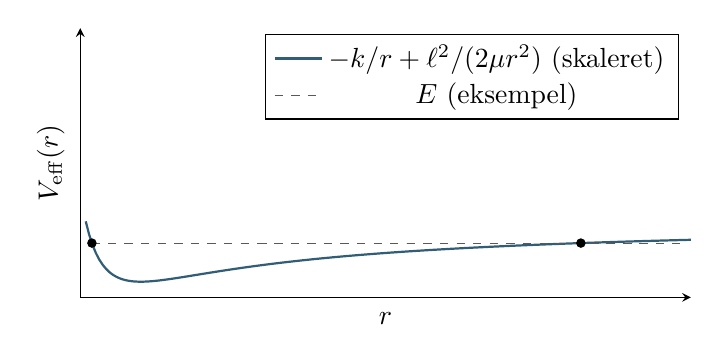
\begin{tikzpicture}\begin{axis}[width=.77\linewidth,height=5cm,axis lines=left,xmin=.45,xmax=6.0,ymin=-.63,ymax=1.6,samples=180,domain=.50:6.0,xlabel={$r$},ylabel={$V_{\rm eff}(r)$},xtick=\empty,ytick=\empty,clip=false]
\addplot[accent,thick]{1/(2*x*x)-1/x};\addlegendentry{$-k/r+\ell^2/(2\mu r^2)$ (skaleret)}
\addplot[black!65,dashed,domain=.55:5.9]{-.18};\addlegendentry{$E$ (eksempel)}
\addplot[only marks,mark=*,mark size=1.5pt] coordinates {(.556,-.18) (5,-.18)};
\end{axis}\end{tikzpicture}\\[-1mm]{\small \itshape Et Kepler-eksempel: skæringer med energilinjen giver de radiale vendepunkter. Figuren er skematisk og dimensionsløs.}\end{center}

\subsection{Cirkulære baner og stabilitet}\label{sec:circular}
Radialligningen er
\[\mu\ddot r=\mu r\dot\phi^2-V'(r)=\frac{\ell^2}{\mu r^3}-V'(r)=-V_{\rm eff}'(r).\]
En cirkelbane har konstant $r=r_0$ og opfylder $V_{\rm eff}'(r_0)=0$. Sæt $r=r_0+\eta$, hvor $|\eta|\ll r_0$. Til første orden gælder
\[\mu\ddot\eta=-V_{\rm eff}''(r_0)\eta,\qquad\boxed{\omega_r^2=\frac{V_{\rm eff}''(r_0)}{\mu}}.\]
\begin{method}Givet $V(r)$: (1) tilføj $\ell^2/(2\mu r^2)$; (2) løs $V_{\rm eff}'(r_0)=0$; (3) indsæt $r_0$ i $V_{\rm eff}''(r_0)$ og undersøg fortegnet. Husk at kontrollere $r_0>0$ og parameterbetingelser.\end{method}
\textbf{Potenspotentiale:} Hvis $V=-a/r^{\alpha}$ med $a>0$, fås fra $V_{\rm eff}'(r_0)=0$
\[\frac{\ell^2}{\mu}=a\alpha r_0^{2-\alpha},\qquad V_{\rm eff}''(r_0)=\frac{\ell^2}{\mu r_0^4}(2-\alpha).\]
Altså er en eksisterende cirkelbane lineært stabil for $0<\alpha<2$ og ustabil for $\alpha>2$ (for $\alpha=2$ kræves særskilt analyse). Dette er \emph{ikke} en Kepler-specifik excentricitetsregel.

\subsection{Binet: fra $r(t)$ til $u(\phi)$}\label{sec:binet}
Sæt $u(\phi)=1/r$ og lad prim betegne afledning efter $\phi$, punkt efter $t$. Under bevaret $\ell\ne0$:
\begin{center}\small\renewcommand{\arraystretch}{1.22}\begin{tabular}{ll}\toprule Størrelse & Omskrivning\\\midrule
$r,\ r^2$ & $1/u,\ 1/u^2$\\
$\dot\phi$ & $\ell u^2/\mu$\\
$\dot r$ & $-(\ell/\mu)u'$\\
$\ddot r$ & $-(\ell^2u^2/\mu^2)u''$\\
$V(r),\ F(r)$ & $V(1/u),\ F(1/u)$\\\bottomrule\end{tabular}\end{center}
Fra kædereglen $\dot r=(\mathrm dr/\mathrm d\phi)\dot\phi$ får man $\dot r=-\ell u'/\mu$. Indsæt i $\mu(\ddot r-r\dot\phi^2)=F(r)$:
\key{u''+u=-\frac{\mu}{\ell^2u^2}F(1/u),\qquad r(\phi)=\frac{1}{u(\phi)}.}
Samtidig er energiudtrykket
\[\boxed{E=\frac{\ell^2}{2\mu}\big[(u')^2+u^2\big]+V(1/u)}.\]
\begin{method}Ud fra en radialkraft: find $F(1/u)$, opstil Binet-ODE'en, klassificér differentialligningen (harmonisk, eksponentiel osv.), løs $u(\phi)$, og brug energien eller begyndelsesdata til at bestemme integrationskonstanter.\end{method}

\subsection{Keplerbaner: energi, excentricitet og banetype}\label{sec:kepler}
\textbf{Kun for} $V(r)=-k/r$, $k>0$, gælder
\[u''+u=\frac{\mu k}{\ell^2},\qquad\boxed{r(\phi)=\frac{p}{1+e\cos(\phi-\phi_0)},\quad p=\frac{\ell^2}{\mu k}},\qquad\boxed{e=\sqrt{1+\frac{2E\ell^2}{\mu k^2}}}.\]
\begin{center}\small\renewcommand{\arraystretch}{1.18}\begin{tabular}{lll}\toprule Energi $E$ & Excentricitet $e$ & Banetype\\\midrule
$E<0$ & $0\le e<1$ & Ellipse (cirkel ved $e=0$)\\
$E=0$ & $e=1$ & Parabel\\
$E>0$ & $e>1$ & Hyperbel\\\bottomrule\end{tabular}\end{center}
\begin{center}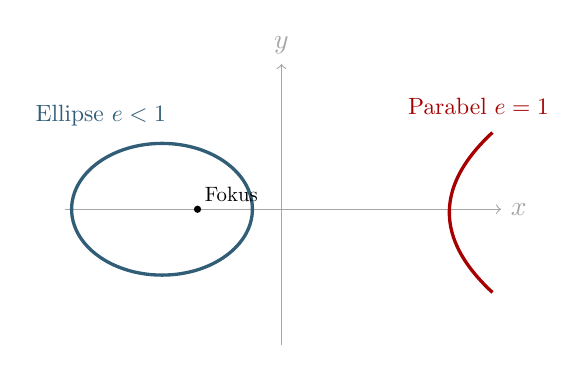
\begin{tikzpicture}[scale=.82]
\draw[->,gray!70] (-3.35,0)--(3.4,0) node[right] {$x$};\draw[->,gray!70] (0,-2.1)--(0,2.25) node[above] {$y$};
\draw[accent,very thick] (-1.85,0) ellipse (1.4 and 1.02);
\fill[black] (-1.3,0) circle(1.6pt) node[above right,scale=.75]{Fokus};
\node[accent,scale=.85] at (-2.8,1.45) {Ellipse $e<1$};
\begin{scope}[xshift=2.05cm,yshift=-.05cm]
\draw[red!65!black,very thick,domain=-1.18:1.18,samples=90] plot ({.55+0.48*\x*\x},{1.05*\x});
\node[red!65!black,scale=.85] at (1.0,1.65) {Parabel $e=1$};
\end{scope}
\end{tikzpicture}\\[-1mm]{\small\itshape Skematisk illustration af keglesnit; hyperblen svarer til $e>1$.}\end{center}
\textbf{Ellipsegeometri:} Kraftcentret ligger i et brændpunkt, ikke i centrum. For en ellipse gælder $r_{\min}=a(1-e)$, $r_{\max}=a(1+e)$ og $b=a\sqrt{1-e^2}$.
\begin{center}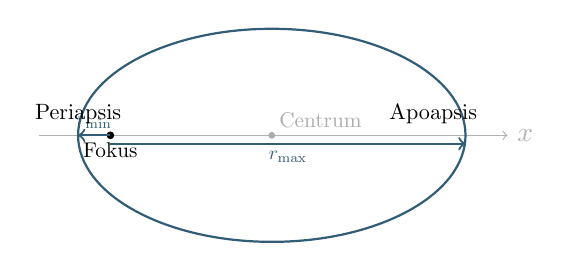
\begin{tikzpicture}[scale=.82]
\draw[->,gray!60](-3.6,0)--(3.65,0) node[right]{$x$};
\draw[accent,thick](0,0) ellipse (3 and 1.65);
\fill[gray!65](0,0) circle (1.5pt) node[above right,scale=.77]{Centrum};
\fill[black](-2.5,0) circle (1.7pt) node[below,scale=.77]{Fokus};
\draw[accent,->,thick](-2.5,0)--(-3,0) node[midway,above,scale=.7]{$r_{\min}$};
\draw[accent,->,thick](-2.5,-.13)--(3,-.13) node[midway,below,scale=.7]{$r_{\max}$};
\node[scale=.8] at (-3.0,.33){Periapsis};\node[scale=.8] at (2.5,.33){Apoapsis};
\end{tikzpicture}\\{\small\itshape Keplerellipsens fokus ligger forskudt fra ellipsens centrum.}\end{center}
\textbf{Ellipseformler:} $E=-k/(2a)$, $r_{\min}=a(1-e)$, $r_{\max}=a(1+e)$, og Keplers tredje lov er $T^2=4\pi^2\mu a^3/k$. Arealloven $\dot A=\ell/(2\mu)$ gælder derimod for enhver central kraft.

\subsection{Udledning og kontrol af excentriciteten}
Med $V=-ku$ og $\dot r=-\ell u'/\mu$ er
\[E=\frac{\ell^2}{2\mu}[(u')^2+u^2]-ku.\]
Sæt $u=(\mu k/\ell^2)(1+e\cos\phi)$ (periapsis ved $\phi=0$):
\[E=\frac{\mu k^2}{2\ell^2}\big[e^2\sin^2\phi+(1+e\cos\phi)^2-2(1+e\cos\phi)\big]=\frac{\mu k^2}{2\ell^2}(e^2-1).\]
Det giver excentricitetsformlen ovenfor. Ellipsens areal $\pi ab$ og $b^2=ap$ sammen med arealhastigheden giver $T^2=4\pi^2\mu a^3/k$.

\subsection{Radialperiode, lukning og præcession}
Hvis der findes to radiale vendepunkter, er vinkelændringen mellem dem
\[\Delta\phi_{1/2}=\int_{r_{\min}}^{r_{\max}}\frac{\ell\,\mathrm dr}{r^2\sqrt{2\mu[E-V_{\rm eff}(r)]}},\qquad\Delta\phi_{\rm radial}=2\Delta\phi_{1/2}.\]
En bane er lukket, når $\Delta\phi_{\rm radial}/(2\pi)$ er rationalt. Ved Keplerpotentialet er den $1$, mens andre centralpotentialer kan give præcession. Forskydning fra én periapsis til den næste er $\Delta\phi_{\rm radial}-2\pi$ ved sammenligning med én fuld omdrejning.

\subsection{Modificeret Keplerpotentiale og præcession}
For $F(r)=-k/r^2+\gamma/r^3$ med $k>0$ svarer potentialet til $V(r)=-k/r+\gamma/(2r^2)$. Binet giver
\[u''+\left(1+\frac{\mu\gamma}{\ell^2}\right)u=\frac{\mu k}{\ell^2}.\]
Sæt $\nu^2=1+\mu\gamma/\ell^2>0$. En oscillerende løsning er
\[\boxed{r(\phi)=\frac{\ell^2\nu^2/(\mu k)}{1+e\cos[\nu(\phi-\phi_0)]}},\qquad
\Delta\phi_{\rm radial}=\frac{2\pi}{\nu}.\]
For $\nu\ne1$ er den næste periapsis generelt forskudt i forhold til én fuld omdrejning; banen er kun lukket for rationelle forhold mellem radial- og vinkelperioderne. Ved en næsten cirkulær bane er $\Delta\phi_{\rm radial}\simeq2\pi\omega_\phi/\omega_r$, hvor $\omega_\phi=\ell/(\mu r_0^2)$.

\subsection{Scattering og virialsætning}
Ved asymptotisk hastighed $v_\infty$ og anslagsparameter $b$ er $E=\tfrac12\mu v_\infty^2$, $\ell=\mu v_\infty b$. For en enkeltvendepunktsbane kan afbøjningsvinklen findes fra
\[\phi_0=\int_{r_{\min}}^\infty\frac{\ell\,\mathrm dr}{r^2\sqrt{2\mu[E-V_{\rm eff}(r)]}},\qquad\Theta=\pi-2\phi_0,\]
med valgt fortegnskonvention. Det differentielle tværsnit er $\mathrm d\sigma/\mathrm d\Omega=(b/\sin\Theta)|\mathrm db/\mathrm d\Theta|$ for én gren; summer over grene, hvis flere $b$ giver samme $\Theta$.
For en bundet Keplerbane med $V=-k/r$ følger særligt $\langle T\rangle=-E$ og $\langle V\rangle=2E$, hvor $E<0$. Virialen $G=\mathbf r\cdot\mathbf p$ er i sig selv generelt ikke bevaret: $G>0$ når afstanden vokser og $G<0$ når den aftager.

For en bundet bevægelse med veldefineret langtidsgennemsnit sættes $G=\vv r\cdot\vv p$, så
\[\frac{\mathrm dG}{\mathrm dt}=2T-\vv r\cdot\nabla V,\qquad2\langle T\rangle=\langle\vv r\cdot\nabla V\rangle.\]
Ved homogent $V\propto r^n$ giver det $2\langle T\rangle=n\langle V\rangle$.

\subsection{Laplace--Runge--Lenz-vektoren}
\begin{center}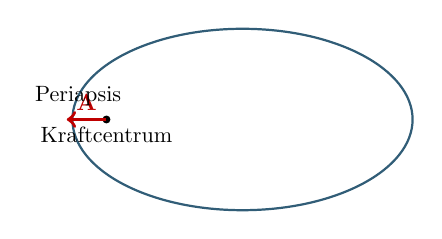
\begin{tikzpicture}[scale=.72]
\draw[accent,thick](0,0) ellipse (3 and 1.6);\fill[black](-2.4,0) circle (2pt) node[below,scale=.8]{Kraftcentrum};
\draw[->,red!75!black,very thick](-2.4,0)--(-3.1,0) node[midway,above,scale=.85]{$\mathbf A$};
\node[scale=.8] at (-2.9,.42){Periapsis};
\end{tikzpicture}\\{\small\itshape Den bevarede Runge--Lenz-vektor peger mod periapsis og fastlægger retningen.}\end{center}
For $V=-k/r$ er den bevarede vektor $\vv A=\vv p\times\vv L-\mu k\hat{\vv r}$ med $|\vv A|=\mu k e$. Da $\dot{\vv p}=-k\vv r/r^3$ og $\dot{\vv L}=0$, fås ved tredobbelt krydsprodukt
\[\dot{\vv p}\times\vv L=\mu k\left(\frac{\dot{\vv r}}r-\frac{\vv r(\vv r\cdot\dot{\vv r})}{r^3}\right)=\mu k\frac{\mathrm d\hat{\vv r}}{\mathrm dt},\]
så $\dot{\vv A}=0$. Desuden er $\vv A\cdot\vv r=\ell^2-\mu kr$, som giver banens polarform med periapsis i retning af $\vv A$.


\clearpage\section{Accelererede og roterende referencesystemer}
\subsection{Accelereret translation}
For et observationssystem med translationsacceleration $\vv a_0$ er den tilsyneladende kraft $-m\vv a_0$.
\subsection{Tidsafledte ved rotation}
For en vektor $\vv A$ og vinkelhastigheden $\vv\Omega$ gælder
\key{\left(\od{\vv A}{t}\right)_{\!I}=\left(\od{\vv A}{t}\right)_{\!R}+\vv\Omega\times\vv A.}
\subsection{Acceleration og fiktive kræfter}
For et system med fast roterende origo og generelt tidsafhængig $\vv\Omega$:
\[\vv a_I=\vv a_R+2\vv\Omega\times\vv v_R+\vv\Omega\times(\vv\Omega\times\vv r)+\dot{\vv\Omega}\times\vv r.\]
\[m\vv a_R=\vv F_{\rm reel}-2m\vv\Omega\times\vv v_R-m\vv\Omega\times(\vv\Omega\times\vv r)-m\dot{\vv\Omega}\times\vv r.\]
De tre led er Coriolis-, centrifugal- og Eulerkraft. Ved et samtidigt accelererende origo tilføjes $-m\vv a_0$.
\subsection{Lagrangefunktion i roterende system}
For inertielt potentiale $V(\vv r,t)$ og $\vv v_I=\vv v_R+\vv\Omega\times\vv r$:
\[\mathcal L_R=\tfrac12m\lvert\vv v_R+\vv\Omega\times\vv r\rvert^2-V.\]
Det kanoniske momentum er $\vv p_R=m(\vv v_R+\vv\Omega\times\vv r)$, ikke nødvendigvis $m\vv v_R$.

\subsection{Udledning af acceleration og praktiske anvendelser}
Transportformlen på den relative hastighed giver $(\dd\vv v_R/\dd t)_I=\vv a_R+\vv\Omega\times\vv v_R$. Produktreglen på $\vv\Omega\times\vv r$ giver
\[\left(\od{}{t}(\vv\Omega\times\vv r)\right)_I=\dot{\vv\Omega}\times\vv r+\vv\Omega\times(\vv v_R+\vv\Omega\times\vv r).\]
Når de to led lægges sammen, optræder $\vv\Omega\times\vv v_R$ to gange, hvilket forklarer Coriolisfaktoren $2$.

\textbf{Jordrotation og frit fald.} For små $\Omega$ kan man ofte først løse den uforstyrrede bane, beregne $-2m\vv\Omega\times\vv v_0$ og derefter integrere denne som en førsteordens korrektion. Vælg akser og breddegrad før krydsproduktet beregnes.

\textbf{Foucaultpendul.} I en lokal vandret plan og under små-udsving-approksimationen er den langsomme præcession proportional med den lodrette komponent $\Omega\sin\lambda$, hvor $\lambda$ er geografisk breddegrad. Fortegn afhænger af halvkugle og aksekonvention.



\clearpage\section{Hamiltonformalismen}
\subsection{Legendretransformation og Hamiltons EOM}
Find $p_i=\partial\mathcal L/\partial\dot q_i$, løs $\dot q_i(q,p,t)$, og definér Hamiltonfunktionen
\key{H(q,p,t)=\sum_i p_i\dot q_i-\mathcal L,\qquad \dot q_i=\pd H{p_i},\quad\dot p_i=-\pd H{q_i}.}
\begin{method}Givet $H$: beregn de to partielle afledte; find $\dot q,\dot p$; hvis opgaven kræver en andenordens EOM, differentier $\dot q$ og eliminer $p$ ved brug af begge Hamiltonligninger. Kontroller ved tilbageindsættelse.\end{method}


\subsubsection*{Hvorfor Legendretransformationen giver Hamiltons ligninger}
Antag en regulær Lagrangefunktion $\mathcal L(q_i,\dot q_i,t)$, hvor $p_i=\partial\mathcal L/\partial\dot q_i$ kan inverteres til $\dot q_i(q,p,t)$. Udgangspunktet er
\[H(q,p,t)=\sum_i p_i\dot q_i-\mathcal L(q,\dot q,t).\]
Produktreglen og det totale differential giver
\begin{align*}
\dd H&=\sum_i\bigl(\dot q_i\,\dd p_i+p_i\,\dd\dot q_i\bigr)-\dd\mathcal L,\\
\dd\mathcal L&=\sum_i\left(\pd{\mathcal L}{q_i}\,\dd q_i+\pd{\mathcal L}{\dot q_i}\,\dd\dot q_i\right)+\pd{\mathcal L}{t}\,\dd t.
\end{align*}
Da $p_i=\partial\mathcal L/\partial\dot q_i$, annullerer leddene med $\dd\dot q_i$ hinanden:
\[\boxed{\dd H=\sum_i\left(\dot q_i\,\dd p_i-\pd{\mathcal L}{q_i}\,\dd q_i\right)-\pd{\mathcal L}{t}\,\dd t.}\]
Men fordi $H=H(q,p,t)$, gælder samtidig
\[\dd H=\sum_i\left(\pd H{q_i}\,\dd q_i+\pd H{p_i}\,\dd p_i\right)+\pd Ht\,\dd t.\]
Sammenligning af koefficienter giver $\partial H/\partial p_i=\dot q_i$, $\partial H/\partial q_i=-\partial\mathcal L/\partial q_i$ og $\partial H/\partial t=-\partial\mathcal L/\partial t$. Med Euler--Lagrange,
$\dd(\partial\mathcal L/\partial\dot q_i)/\dd t=\partial\mathcal L/\partial q_i$, fås derfor
\key{\dot q_i=\pd H{p_i},\qquad\dot p_i=-\pd H{q_i}.}
Dette er samme metode i et variationsproblem med $\mathcal L\to f$, $H\to g$, $q\to y$, $p\to z$ og $t\to x$.


\subsubsection*{Fire trin: den omvendte hastighed--impuls-relation}
\begin{method}\textbf{1.} Differentier den givne $\mathcal L(q,\dot q,t)$: $p_i=\partial\mathcal L/\partial\dot q_i$. \textbf{2.} Isolér $\dot q_i=\dot q_i(q,p,t)$ \emph{fra impulsligningen}. \textbf{3.} Indsæt hastighederne alle steder i $H=\sum_i p_i\dot q_i-\mathcal L$, også inde i $\mathcal L$. \textbf{4.} Find eventuelt EOM fra $\dot q_i=\partial H/\partial p_i$ og $\dot p_i=-\partial H/\partial q_i$.\end{method}
For $\mathcal L=\tfrac12m\dot q^2+a(q,t)\dot q-V(q,t)$:
\[p=m\dot q+a(q,t)\ \Rightarrow\ \dot q=\frac{p-a(q,t)}m\ \Rightarrow\ \boxed{H=\frac{[p-a(q,t)]^2}{2m}+V(q,t)}.\]
\textbf{Kædereglen:} Ved $\partial H/\partial q$ holdes $p,t$ faste; ved $\partial H/\partial p$ holdes $q,t$ faste. Ved total tidsafledning indgår også $q(t)$: $\mathrm d[tV'(q(t))]/\mathrm dt=V'(q)+tV''(q)\dot q$. Den almindelige Legendretransformation kræver, at impulsligningerne kan inverteres lokalt.

\subsection{Legendretransformationen i et konkret mekanisk system}
For $\mathcal L=\tfrac12m\dot q^2-V(q)$ er $p=m\dot q$. Inversion giver $\dot q=p/m$ og dermed
\[H(q,p)=p\frac pm-\left(\frac12m\frac{p^2}{m^2}-V(q)\right)=\frac{p^2}{2m}+V(q).\]
Hamiltonligningerne bliver $\dot q=p/m$, $\dot p=-V'(q)$, så $m\ddot q=-V'(q)$; dette er en direkte konsistenskontrol. Hvis Hessianen $\partial^2\mathcal L/\partial\dot q_i\partial\dot q_j$ er singulær, kan hastighederne ikke nødvendigvis elimineres, og den almindelige Legendretransformation er ikke regulær.

\subsection{Tidsudvikling og bevarelse}
For $F(q,p,t)$ langs Hamiltons bevægelse gælder
\[\od Ft=\PB FH+\pd Ft,\qquad \od Ht=\pd Ht.\]
En størrelses $F$ bevarelse kræver $\PB FH+\partial F/\partial t=0$ langs bevægelsen.
\subsection{Find de oplagte bevarede størrelser fra Hamiltonfunktionen}\label{sec:ham-constants}
En Hamiltonfunktion er ikke blot en alternativ bevægelsesligning: dens afhængighed af koordinater og tid viser straks mulige integraler. For autonome kanoniske systemer gælder
\[
\dot p_i=-\frac{\partial H}{\partial q_i},\qquad
\frac{\dd H}{\dd t}=\frac{\partial H}{\partial t}.
\]
Dermed giver $\partial H/\partial q_i=0$ en bevaret \emph{kanonisk impuls} $p_i$; $\partial H/\partial t=0$ giver en bevaret \emph{Hamiltonfunktion}. Ingen af udsagnene kræver, at $H$ er lig den mekaniske energi $T+V$. Dette skal kontrolleres særskilt ud fra Legendretransformationens antagelser og eventuel tidsafhængighed.
\begin{method}Start altid med $H(q,p,t)$: (1) kontrollér hvilke $q_i$ der mangler, så $\dot p_i=0$; (2) undersøg eksplicit tidsafhængighed, så $\dd H/\dd t=\partial H/\partial t$; (3) undersøg translationer/rotationer via deres generatorer; (4) hvis ingen oplagte integraler er nok, gå til Poissonparentes-testen og ansatzmetoden i afsnit~\ref{sec:find-conserved}. Skeln mellem konserveret $H$ og fysisk energi.\end{method}

\subsection{Hamiltons ligninger på matrixform og fasevirkningen}
Med $z=(q_1,\dots,q_n,p_1,\dots,p_n)^T$ og $J=\bigl(\begin{smallmatrix}0&I\\-I&0\end{smallmatrix}\bigr)$:
\[\dot z=J\nabla_z H,\qquad S[q,p]=\int\left(\sum_i p_i\dot q_i-H\right)\dd t.\]


\subsection{Roterende Hamiltonfunktion}
Når rotationshastigheden er konstant og $\vv p_R=m(\vv v_R+\vv\Omega\times\vv r)$, giver Legendretransformationen
\[H_R=\vv p_R\cdot\vv v_R-\mathcal L_R=\frac{|\vv p_R|^2}{2m}+V-\vv\Omega\cdot(\vv r\times\vv p_R).\]
Altså $H_R=H_{\rm inertiel}-\vv\Omega\cdot\vv L$ i den tilsvarende kanoniske beskrivelse. For eksplicit tidsafhængig $\vv\Omega$ kræves særlig omhu med koordinattransformationen og potentiellets tidsafhængighed.

\subsection{Udledning af Hamiltons ligninger fra fasevirkningen}
Variér $S[q,p]=\int_{t_1}^{t_2}(\sum_i p_i\dot q_i-H)\,\dd t$, med $\delta q_i(t_1)=\delta q_i(t_2)=0$ og uafhængige variationer $\delta p_i$:
\[\delta S=\int\sum_i\left[\delta p_i\dot q_i+p_i\delta\dot q_i-\pd H{q_i}\delta q_i-\pd H{p_i}\delta p_i\right]\dd t.\]
Ved integration ved dele af $p_i\delta\dot q_i$ forsvinder randleddene, og
\[\delta S=\int\sum_i\left[\left(\dot q_i-\pd H{p_i}\right)\delta p_i-\left(\dot p_i+\pd H{q_i}\right)\delta q_i\right]\dd t.\]
Uafhængigheden af variationerne giver Hamiltons to ligninger.



\clearpage\section{Kanoniske transformationer og Poissonparenteser}
\subsection{Definition og Kroneckers delta}\label{sec:canon}
En lokalt invertibel transformation $(q,p)\mapsto(Q,P)$ er kanonisk, hvis de fundamentale Poissonparenteser bevares:
\key{\PB{Q_i}{Q_j}=0,\qquad\PB{P_i}{P_j}=0,\qquad\PB{Q_i}{P_j}=\delta_{ij}.}
Kroneckers delta er $\delta_{ij}=1$ for $i=j$ og $0$ for $i\ne j$. Ved den direkte test af $(Q,P)$ beregnes parenteserne i de \emph{gamle} variable $(q,p)$. For den inverse transformation kan man i stedet teste de gamle variable i de nye kanoniske variable.
\begin{note}\textbf{Ét koordinatpar:} $\{Q,Q\}=\{P,P\}=0$ automatisk; kontrollér kun $\{Q,P\}=Q_qP_p-Q_pP_q=1$.\end{note}
\begin{method}\textbf{Vælg det sæt, funktionerne er udtrykt ved.} Hvis $Q=Q(q,p)$ og $P=P(q,p)$ er opgivet, beregn
\[\PB QP_{q,p}=\pd Qq\pd Pp-\pd Qp\pd Pq=1.\]
Hvis der i stedet er opgivet $q=q(Q,P)$ og $p=p(Q,P)$, beregn
\[\PB qp_{Q,P}=\pd qQ\pd pP-\pd qP\pd pQ=1.\]
For \emph{én frihedsgrad} og en lokalt invertibel transformation er testene ækvivalente. For flere frihedsgrader skal alle de fundamentale parenteser testes, enten for den direkte eller for den inverse transformation. Bland ikke afledte med hensyn til forskellige koordinatsæt.\end{method}
\textbf{To koordinatpar:} Kontrollér de seks uafhængige relationer
\[\PB{Q_1}{P_1}=\PB{Q_2}{P_2}=1,\qquad\PB{Q_1}{P_2}=\PB{Q_2}{P_1}=0,\]
\[\PB{Q_1}{Q_2}=\PB{P_1}{P_2}=0.\]
Hver parentes rummer summen over $k=1,2$ af afledte i $(q_k,p_k)$.
\subsection{Poissonparenteser og regneregler}\label{sec:pb}
\key{\PB FG=\sum_{k=1}^n\left(\pd F{q_k}\pd G{p_k}-\pd F{p_k}\pd G{q_k}\right).}
\[\PB F{q_i}=-\pd F{p_i},\qquad\PB F{p_i}=\pd F{q_i},\qquad\PB FG=-\PB GF.\]
\begin{note}Eksempel fra rotationsgeneratoren, jf. afsnit~\ref{sec:angular}: $L_x=yp_z-zp_y$, derfor $\{L_x,y\}=-\partial L_x/\partial p_y=z$ og $\{L_x,p_y\}=\partial L_x/\partial y=p_z$.\end{note}
\subsection{Genererende funktioner: fire typer}
Alle fire typer antages at definere en lokalt invertibel kanonisk transformation. I en standardkonvention:
\begin{center}\begin{tabular}{llll}\toprule Type & Variable & Gammel impuls/koordinat & Ny impuls/koordinat\\\midrule
$F_1$&$(q,Q,t)$&$p=\partial_qF_1$&$P=-\partial_QF_1$\\
$F_2$&$(q,P,t)$&$p=\partial_qF_2$&$Q=\partial_PF_2$\\
$F_3$&$(p,Q,t)$&$q=-\partial_pF_3$&$P=-\partial_QF_3$\\
$F_4$&$(p,P,t)$&$q=-\partial_pF_4$&$Q=\partial_PF_4$\\\bottomrule\end{tabular}\end{center}
For alle typer er $K=H+\partial F_a/\partial t$ med den afledte taget ved fastholdte \emph{uafhængige argumenter til den valgte type}.
\subsubsection*{Genererende funktioner skrevet med Leibniz-notation}
\[\begin{aligned}
F_1(q,Q,t):\quad &p_i=\pd{F_1}{q_i}, &P_i&=-\pd{F_1}{Q_i},\\
F_2(q,P,t):\quad &p_i=\pd{F_2}{q_i}, &Q_i&=\pd{F_2}{P_i},\\
F_3(p,Q,t):\quad &q_i=-\pd{F_3}{p_i}, &P_i&=-\pd{F_3}{Q_i},\\
F_4(p,P,t):\quad &q_i=-\pd{F_4}{p_i}, &Q_i&=\pd{F_4}{P_i}.
\end{aligned}\]
\begin{method}\textbf{Kontrollér en given genererende funktion.} Find typen ud fra dens uafhængige argumenter; differentier med hensyn til begge argumenter; sammenlign de resulterende udtryk med den ønskede transformation. For eksempel kræver $S(q,P,t)$, at $p=\partial S/\partial q$ og $Q=\partial S/\partial P$. Tidsleddet $\partial S/\partial t$ bestemmer derimod ændringen af Hamiltonfunktionen og tester ikke alene transformationen.\end{method}
\begin{method}\textbf{Løs bevægelsen via en kanonisk transformation.} Omskriv $H(q,p,t)$ til $\widetilde H(Q,P,t)$, løs $\dot Q=\partial\widetilde H/\partial P$ og $\dot P=-\partial\widetilde H/\partial Q$, og indsæt derefter $Q(t),P(t)$ i $q(Q,P,t),p(Q,P,t)$.\end{method}
\subsection{Den transformerede Hamiltonfunktion}\label{sec:newH}
\begin{method}\textbf{1.} Identificér transformationen og den korrekte genererende funktion $F_a$. \textbf{2.} Beregn $\partial F_a/\partial t$ ved fastholdte argumenter. \textbf{3.} Invertér for $q=q(Q,P,t)$ og $p=p(Q,P,t)$. \textbf{4.} Indsæt begge i den oprindelige $H$ og tilføj tidsleddet.\end{method}
\key{\widetilde H(Q,P,t)=H(q,p,t)+\left.\pd{F_a}{t}\right|_{\text{egne argumenter}}.}
Her skal højresiden til sidst omskrives til $(Q,P,t)$. Hvis $F_a$ er \emph{eksplicit} tidsuafhængig, er tidsleddet nul, men $H$ skal stadig omskrives til $(Q,P)$.
\textbf{Mini-eksempel.} For $Q=aq$, $P=p/a$ med konstant $a\ne0$ og $H=p^2/(2m)+kq^2/2$ fås $q=Q/a$, $p=aP$, og
\[K(Q,P)=\frac{a^2P^2}{2m}+\frac{kQ^2}{2a^2}.\]
\begin{note}Tidsafhængige kanoniske transformationer kræver omhu: $\partial F/\partial t$ er ikke den totale afledte $\dd F/\dd t$.\end{note}


\subsubsection*{Omvendt opgavetype: find $F$ fra den ønskede $\widetilde H$}
\begin{method}\textbf{1.} Undersøg, om man kan vælge $\partial F/\partial t=0$ og dermed $\widetilde H=H$. Det er et muligt valg, ikke en almen regel. \textbf{2.} Brug den ønskede $\widetilde H$ til at vælge nye variable, fx $P=H$ hvis $\widetilde H=P$. \textbf{3.} Identificér $F_1$--$F_4$ og isolér den gamle variabel, der passer til dens argumenter. \textbf{4.} Integrér den tilhørende transformationsrelation og husk en vilkårlig funktion af de andre argumenter. \textbf{5.} Differentier for at bestemme den anden nye variabel, og kontrollér begge relationer samt $\widetilde H=H+F_t$.\end{method}
Eksempel: $H=p^2/(2m)+mgq$, ønsket $\widetilde H=P$ og en type 4-funktion $U(p,P)$. Vælg $U_t=0$ og $P=H$, så
\[q=\frac{P}{mg}-\frac{p^2}{2m^2g},\quad q=-U_p\quad\Rightarrow\quad\boxed{U(p,P)=-\frac{pP}{mg}+\frac{p^3}{6m^2g}+f(P)},\]
\[Q=U_P=-\frac{p}{mg}+f'(P).\]
Vælg eksempelvis $f=0$; $\{Q,P\}_{q,p}=1$. En direkte integration af $F_t=\widetilde H-H$ er generelt utilstrækkelig, fordi den ukendte transformation også bestemmer $q,p$ på højresiden.

\subsection{Oprindelse af de genererende funktioner}
En kanonisk transformation bevarer Hamiltons variationsprincip, hvis fase-rummets én-former opfylder
\[\sum_i p_i\,\dd q_i-H\,\dd t=\sum_i P_i\,\dd Q_i-K\,\dd t+\dd F_1(q,Q,t).\]
Sammenligning af koefficienterne foran $\dd q_i$, $\dd Q_i$ og $\dd t$ giver $p_i=\partial F_1/\partial q_i$, $P_i=-\partial F_1/\partial Q_i$ og $K=H+\partial F_1/\partial t$.
Ved Legendreomformninger fås $F_2=F_1+\sum_iP_iQ_i$, $F_3=F_1-\sum_i p_iq_i$ og $F_4=F_1+\sum_iP_iQ_i-\sum_i p_iq_i$; dette forklarer fortegnstabellen ovenfor.
\subsection{Symplektisk Jacobimatrix}
Sæt $z=(q,p)^T$, $Z=(Q,P)^T$, $M=\partial Z/\partial z$, $J=\left(\begin{smallmatrix}0&I\\-I&0\end{smallmatrix}\right)$. Den kompakte kanonicitetsbetingelse er
\[\boxed{MJM^T=J.}\]
Dette er ækvivalent med samtlige fundamentale Poissonparentesbetingelser. Under standardantagelser følger også $M^TJM=J$.

\subsection{Rotationsgeneratorer og bevarelse}
Den mekaniske rotationsgenerator i kanoniske kartesiske variable har $\vv L=\vv r\times\vv p$ for sædvanlige systemer; så $\PB{L_x}{y}=z$, $\PB{L_x}{z}=-y$, $\PB{L_x}{p_y}=p_z$. \emph{Generatorvirkningen} skal ikke forveksles med \emph{bevarelse}: for en tidsuafhængig rotationsinvariant $H$ er $\PB{L_x}{H}=0$, og dermed er $L_x$ bevaret.


\clearpage\section{Hamilton--Jacobi-teori}\label{sec:hj}
\textbf{Fra kanoniske transformationer til løsning af bevægelsen.} I kapitel~\ref{sec:canon} fandt vi, hvordan man kan ændre fasevariable uden at ændre den fysiske bane. Kan vi vælge generatoren så godt, at den \emph{nye Hamiltonfunktion er nul}? Hvis $K(Q,P,t)=0$, giver Hamiltons ligninger straks
\[
\dot Q_i=\frac{\partial K}{\partial P_i}=0,\qquad
\dot P_i=-\frac{\partial K}{\partial Q_i}=0.
\]
De nye variable er således konstanter. Hamilton--Jacobi-teorien (HJ) er metoden til at \emph{finde denne transformation} ved at løse en partiel differentialligning for dens generator.

\subsection{Hovedfunktionen og udledningen af HJ-ligningen}\label{sec:hj-equation}
Vælg en tidsafhængig generator af type 2 med egne argumenter $(q,P,t)$:
\[
F_2(q,P,t)=S(q,P,t).
\]
Fra afsnit~\ref{sec:gen-legendre} ved vi, at
\[
p_i=\frac{\partial S}{\partial q_i},\qquad
Q_i=\frac{\partial S}{\partial P_i},\qquad
K=H(q,p,t)+\left.\frac{\partial S}{\partial t}\right|_{q,P}.
\]
Vælg $S$ sådan, at $K=0$. Efter substitution af $p_i=\partial S/\partial q_i$ fås
\key{H\left(q_1,\ldots,q_n,
\frac{\partial S}{\partial q_1},\ldots,\frac{\partial S}{\partial q_n},t\right)
+\frac{\partial S}{\partial t}=0.}
Funktionen $S$ kaldes \emph{Hamiltons hovedfunktion}. Dens gradient giver de gamle impulser, mens dens parameterafledte giver de nye koordinater. Bemærk, at $\partial S/\partial t$ beregnes ved faste $q,P$; den er ikke $\dd S/\dd t$ langs en bane. HJ er en \emph{førsteordens partiel differentialligning} i $(q,t)$, selv om Hamiltons oprindelige bevægelse kan omfatte mange koblede differentialligninger.

Samtidig gælder for den oprindelige fasevirkning langs en løsning
\[
\frac{\dd S}{\dd t}=
\sum_i\frac{\partial S}{\partial q_i}\dot q_i+\frac{\partial S}{\partial t}
=\sum_i p_i\dot q_i-H,
\]
når $P$ holdes konstant. Dermed er hovedfunktionen (op til passende rand- og integrationskonstanter) virkningen evalueret langs den klassiske bevægelse. Dette er den konkrete forbindelse til fasevirkningen fra kapitel~5.

\subsection{Tidsuafhængig Hamiltonfunktion: $S$ versus $W$}
Hvis $H(q,p)$ ikke afhænger eksplicit af $t$, kan man forsøge at separere tiden:
\[
S(q,\alpha,t)=W(q,\alpha)-Et.
\]
Her er $E$ en separationskonstant, der i den autonome opgave er Hamiltonfunktionens konstante værdi; for $n$ frihedsgrader kan de øvrige $n-1$ uafhængige parametre også indgå i $\alpha$. HJ-ligningen bliver
\key{H\left(q,\frac{\partial W}{\partial q}\right)=E.}
$W$ kaldes \emph{Hamiltons karakteristiske funktion}; den er den rumlige del af $S$, ikke en ny Hamiltonfunktion. Ved en frihedsgrad med
$H=p^2/(2m)+V(q)$ løses først
\[
\frac{\partial W}{\partial q}
=p(q,E)=\pm\sqrt{2m[E-V(q)]},
\]
og derpå
\[
\boxed{W(q,E)=\pm\int^q\sqrt{2m[E-V(s)]}\,\dd s.}
\]
Fortegnet vælges for den relevante impulsgren. Integralet er reelt, hvor $E\ge V(q)$; et vendepunkt kan kræve en ny gren. Ved flervariabel separation $W=\sum_iW_i(q_i;\alpha)$ er dette en \emph{ansats}, som skal kontrolleres ved tilbageindsættelse. Den er ikke mulig for alle Hamiltonfunktioner.

\subsection{Et fuldstændigt integral og rekonstruktion af bevægelsen}
Det er ikke tilstrækkeligt at finde én funktion, der opfylder HJ-ligningen: vi skal også udlede \emph{den fysiske bane}. Et \emph{partikulært integral} er en enkelt løsning af HJ, mens et \emph{fuldstændigt integral} $S(q,\alpha,t)$ lokalt indeholder $n$ uafhængige parametre $\alpha_i$, sådan at den blandede afledte matrix er regulær:
\key{\det\left(\frac{\partial^2S}{\partial q_i\partial\alpha_j}\right)\ne0.}
Denne betingelse gør det muligt lokalt at bruge $S$ som en type 2-generator og rekonstruere løsningen via
\[
\boxed{p_i(t)=\frac{\partial S}{\partial q_i},\qquad
\beta_i=Q_i=\frac{\partial S}{\partial\alpha_i},\qquad
P_i=\alpha_i.}
\]
Da $K=0$, er \emph{både} $\alpha_i$ og $\beta_i$ konstante. For givne initialdata $(q(t_0),p(t_0))$ bestemmes de ved de to sæt relationer ved $t_0$; derefter løses $\beta_i=\partial S/\partial\alpha_i$ for $q_i(t)$, og impulserne findes fra $\partial S/\partial q_i$. Regularitetsbetingelsen er lokal; ved kaustikker, vendepunkter eller koordinatsingulariteter må man ofte skifte gren eller koordinatkort.

For $S=W(q,E,\ldots)-Et$ giver afledning efter energiparameteren
\[
\beta_E=\frac{\partial S}{\partial E}
=\left.\frac{\partial W}{\partial E}\right|_q-t,
\quad\text{altså}\quad
\boxed{\frac{\partial W}{\partial E}=t+\beta_E.}
\]
Her skal $q$ og de øvrige parametre holdes faste ved den partielle afledte. Andre parametre giver tilsvarende $\beta_j=\partial W/\partial\alpha_j$. Energien bestemmer ikke automatisk alle øvrige konstanter eller den valgte fortegnsgren.

\begin{method}\textbf{Tidsuafhængig HJ:} (1) kontroller $\partial H/\partial t=0$ og vælg $S=W-Et$; (2) erstat \emph{alle} $p_i$ med $\partial W/\partial q_i$; (3) separér, hvis strukturen tillader det, og integrér for $W$ med de nødvendige parametre; (4) differentier $S$ efter parametrene ved faste $q$; (5) bestem $\alpha_i,\beta_i$ fra initialdata og løsningens domæne; (6) løs for $q(t)$, beregn $p(t)$ og verificér Hamiltons ligninger.\end{method}

\subsection{Fri partikel: et helt HJ-forløb}
Tag $H(q,p)=p^2/(2m)$. En særlig bekvem \emph{fuldstændig} type 2-generator med parameter $P$ er
\[
S(q,P,t)=qP-\frac{P^2}{2m}t.
\]
Den opfylder
\[
\frac1{2m}\left(\frac{\partial S}{\partial q}\right)^2+
\frac{\partial S}{\partial t}
=\frac{P^2}{2m}-\frac{P^2}{2m}=0,
\qquad
\frac{\partial^2S}{\partial q\partial P}=1\ne0.
\]
De gamle og nye variable er
\[
p=\frac{\partial S}{\partial q}=P,\qquad
Q=\frac{\partial S}{\partial P}=q-\frac Pm t.
\]
Med $P=P_0$ og $Q=Q_0$ konstante finder vi
\[
\boxed{p(t)=P_0,\qquad q(t)=Q_0+\frac{P_0}{m}t.}
\]
Dette demonstrerer hele idéen: HJ-generatoren flytter tidsudviklingen ind i en eksplicit tidsafhængig koordinattransformation. Energi $E=P_0^2/(2m)$ fastlægger kun $|P_0|$, ikke fortegnet; begyndelsesdata afgør retningen.

\subsection{Tidsafhængige Hamiltonfunktioner og separation}
Når $H(q,p,t)$ afhænger eksplicit af tiden, kan man normalt \emph{ikke} sætte $S=W-Et$, men den fulde PDE gælder stadig:
\[
H\left(q,\frac{\partial S}{\partial q},t\right)+\frac{\partial S}{\partial t}=0.
\]
En tidsafhængig separationsansats kan være mulig i særlige modeller, men skal begrundes. Et simpelt kontroleksempel er $H(q,p,t)=p^2/(2m)+f(t)$, hvor
\[
S(q,P,t)=qP-\frac{P^2}{2m}t-\int^t f(\tau)\,\dd\tau
\]
opfylder HJ, giver $p=P$ og $Q=q-Pt/m$. Det rene tidsled i $H$ påvirker generatoren, men ikke de klassiske bevægelsesligninger for $q,p$.
\begin{method}\textbf{Tidsafhængig HJ:} Start fra den fulde PDE, vælg kun en ansats hvis den er konsistent med tidsleddene, find et regulært fuldstændigt integral, bestem $Q_i=\partial S/\partial P_i$, og kontrollér både PDE'en, Hamiltons ligninger og den valgte tids- og parameterg ren.\end{method}

\subsection{HJ efter en tidsafhængig kanonisk transformation: eksamen 2020.1}\label{sec:hj-2020}
Den oprindelige eksamen 2020, opgave 1, begynder med den dæmpede oscillator
\[
\mathcal L(q,\dot q,t)=\frac12e^{\mu t/m}(m\dot q^2-kq^2),
\qquad m,\mu,k>0.
\]
En \emph{første} tidsafhængig generator $F_2(q,P,t)=e^{\mu t/(2m)}qP$ giver
$Q=e^{\mu t/(2m)}q$ og den tidsuafhængige Hamiltonfunktion
\[
\widetilde H(Q,P)=\frac{P^2}{2m}+\frac{kQ^2}{2}+
\frac{\mu}{2m}QP.
\]
Der ønskes nu en \emph{anden} kanonisk transformation med $K=0$, fundet fra HJ. Vi arbejder derfor med de mellemliggende \emph{nye} koordinater $(Q,P)$; HJ skal differentieres med hensyn til $Q$, ikke den oprindelige $q$.
Vælg $S_{\mathrm{HJ}}(Q,E,t)=W(Q,E)-Et$. Sæt
$P=\partial W/\partial Q$ og brug energiligningen
\[
\frac1{2m}\left(\frac{\partial W}{\partial Q}\right)^2+
\frac{\mu Q}{2m}\frac{\partial W}{\partial Q}
+\frac{kQ^2}{2}=E.
\]
Gang med $2m$ og fuldend kvadratet:
\[
\left(W_Q+\frac{\mu Q}{2}\right)^2
=2mE-\left(mk-\frac{\mu^2}{4}\right)Q^2.
\]
For $k>\mu^2/(4m)$ defineres $\omega^2=k/m-\mu^2/(4m^2)>0$, så
\[
W_Q=-\frac{\mu Q}{2}
\pm\sqrt{2mE-m^2\omega^2Q^2},
\]
og dermed
\key{W(Q,E)=-\frac{\mu Q^2}{4}
\pm\int^Q\sqrt{2mE-m^2\omega^2s^2}\,\dd s.}
Denne udledning er indholdet af eksamen 2020.1d; udtrykket er lokalt gyldigt på en gren, hvor kvadratroden er reel.

I opgave 1e bestemmes bevægelsen fra \emph{parameterafledningen}, ikke fra $W$ alene:
\[
\beta=\frac{\partial S_{\mathrm{HJ}}}{\partial E}
=\pm\int^Q\frac{m\,\dd s}{\sqrt{2mE-m^2\omega^2s^2}}-t.
\]
Sæt $A=\sqrt{2E/(m\omega^2)}$. Integralet giver på en valgt gren
\[
t+\beta=\pm\frac1\omega\arcsin\left(\frac QA\right).
\]
Efter valg af fase og korrekt stykvis fortsættelse fås
\[
Q(t)=A\cos(\omega t+\varphi_0),\qquad
\boxed{q(t)=A e^{-\mu t/(2m)}\cos(\omega t+\varphi_0).}
\]
$E$ er her den \emph{konstante værdi af den transformerede} $\widetilde H$, ikke uden videre den oprindelige oscillators bevarede mekaniske energi. Startposition og starthastighed bestemmer $A,\varphi_0$ på den fysiske gren. Tilbage-transformationen er nødvendig; uden den mangler dæmpningen.
\begin{method}Ved en forudgående transformation: (1) brug den transformerede Hamiltonfunktion og \emph{dens} koordinater i HJ; (2) fuldend eventuelt kvadratet, find $W_Q$, integrér; (3) brug $\partial W/\partial E=t+\beta$ til tiden; (4) transformér helt tilbage til de oprindelige variable; (5) verificér den oprindelige bevægelsesligning og initialdata.\end{method}

\subsection{Periodiske bevægelser og aktionsvariable: eksamen 2021.4}
\textbf{Afgrænsning.} Eksamen 2021, opgave 4, bruger \emph{aktions- og vinkelvariable} for periodiske bevægelser, ikke den samme opgave som den direkte HJ-separation i 2020.1. Begrebet hænger sammen med $W$, fordi den klassiske impuls $p=\partial W/\partial q$ kan integreres over en fuld periode. Med eksamenssættets konvention defineres \emph{aktionen}
\[
\boxed{J(E)=\oint p(q,E)\,\dd q,\qquad
\nu=\frac{\partial H(J)}{\partial J}=\frac1T.}
\]
$\nu$ måles i omløb pr.\ tid; den tilhørende vinkelhastighed er $2\pi\nu$. Refleksioner ved hårde vægge behandles stykkevist; HJ-generatoren er ikke ét globalt glat udtryk gennem kollisionerne.

\textbf{2021.4a: fri partikel mellem to vægge.} En masse $m$ bevæger sig mellem $x=0$ og $x=L$ og reflekteres elastisk. På de to grene er $p=\pm\sqrt{2mE}$, og
\[
J=\oint p\,\dd x=2L\sqrt{2mE},\qquad
\boxed{H(J)=\frac{J^2}{8mL^2}}.
\]
Dermed er
\[
\nu=\frac{\partial H}{\partial J}
=\frac{J}{4mL^2}
=\frac{|p|}{2mL}.
\]
Det er netop den inverse tid for frem-og-tilbage-bevægelsen $T=2L/(|p|/m)$.

\textbf{2021.4b: frit fald og elastisk refleksion.} En partikel tabes fra højden $h$ og spejles ved jorden. For $E=mgh$ er den positive gren
$p(x,E)=\sqrt{2m(E-mgx)}$. Derfor
\begin{align*}
J(E)&=2\int_0^{E/(mg)}\sqrt{2m(E-mgx)}\,\dd x\\
&=\frac{4\sqrt{2m}}{3mg}E^{3/2},
\end{align*}
og omskrivning giver
\[
\boxed{H(J)=\left(\frac{3g}{4}\sqrt{\frac m2}\,J\right)^{2/3}.}
\]
Differentiér efter $J$ og indsæt $E=mgh$:
\[
\boxed{\nu=\frac{\partial H}{\partial J}
=\frac12\sqrt{\frac{g}{2h}}.}
\]
Dette stemmer med den direkte fald-og-retur-tid $T=2\sqrt{2h/g}$. Begge eksempler demonstrerer, at et \emph{aktionsintegral} kan bestemme periodetiden uden at løse $x(t)$ eksplicit.
\begin{method}Ved periodiske 1D-problemer: identificér de to grene af $p(q,E)$, beregn $J=\oint p\,\dd q$ med korrekt orientering, isolér $H(J)$ og find $\nu=\partial H/\partial J$. Ved hårde refleksioner opdeles integralet i glatte stykker. Kontrollér ved at beregne den direkte periodetid.\end{method}

\subsection{Samlet metodevalg og forbindelse til kanoniske transformationer}
\begin{method}
\textbf{HJ for tidsuafhængigt $H$:} Sæt $S=W-Et$, løs $H(q,\partial_qW)=E$ og find banen fra $\partial W/\partial E=t+\beta_E$. \textbf{HJ for tidsafhængigt $H$:} Løs hele $H(q,\partial_qS,t)+S_t=0$ og brug et regulært fuldstændigt integral. \textbf{Efter en forudgående transformation:} Brug dens nye koordinater og transformér tilbage til sidst. \textbf{Periodisk bevægelse:} Overvej $J=\oint p\,\dd q$ og $\nu=\partial H/\partial J$. Alle metoder kræver kontrol af grene, integrationskonstanter, regularitet og de oprindelige bevægelsesligninger.
\end{method}
Hamilton--Jacobi er således ikke en konkurrerende fysisk teori: den bruger præcis de kanoniske transformationer fra foregående kapitel til at vælge en beskrivelse, hvor dynamikken ligger i selve transformationen og de nye variable er konstanter.

\clearpage\section{Hurtigt metodevalg til eksamen}
\begin{center}\begin{tabular}{p{49mm}p{93mm}}\toprule Når opgaven spørger om \dots & Start her\\\midrule
EOM ud fra $\mathcal L$ & Euler--Lagrange, afsnit 2.1\\
EOM ud fra $H$ & To Hamiltonligninger, afsnit 5.1\\
Konserveret impuls eller energi & Cyklisk koordinat / tidssymmetri, afsnit 2.3 og 2.5\\
Bindingskraft & Multiplikatorer, afsnit~\ref{sec:lambda} (2.9)\\
Central bane $r(\phi)$ & Binetligningen, afsnit~\ref{sec:binet} (3.2)\\
Radial stabilitet & $V_{\rm eff}'=0$, $V_{\rm eff}''>0$, afsnit~\ref{sec:veff} (3.2)\\
Kanonisk transformationskontrol & Fundamental PB-test, afsnit~\ref{sec:canon}\\
Ny Hamiltonfunktion efter skift & Invertér $(Q,P)$ og anvend afsnit~\ref{sec:newH}\\
Poissonparenteser med $L_i$ & Kartesiske $L_i$, afsnit~\ref{sec:angular} og~\ref{sec:pb}\\
Bevarede størrelser fra $H$ & Manglende $q_i$ og eksplicit tid: afsnit~\ref{sec:ham-constants}.\\
Mindre oplagte bevarede størrelser & Poisson-test, generator og ansatz: afsnit~\ref{sec:find-conserved}.\\
Coriolis-afbøjning & Afsnit 4.8: 0.-ordensbane og førsteordensintegration.\\
Hamilton--Jacobi-funktion & HJ-ligning, separation og tilbage-transformation, afsnit~\ref{sec:hj}.\\\bottomrule\end{tabular}\end{center}


\end{document}
